\section{Introduction}
\label{section:introduction}

\Glspl{llm} such as GPT-4 \citep{openai2023gpt4}, Claude \citep{anthropic2024claude}, Gemini \citep{gemini2023}, and Llama \citep{grattafiori2024llama3} show broad competence across reasoning, code, and multilingual tasks, at a cost that scaling laws \citep{kaplan2020scaling,hoffmann2022chinchilla} made predictable but not small: multi-thousand-GPU training runs, tens of gigabytes of accelerator memory per served replica, and a network round trip, a per-token charge, and a transfer of prompt content for every call. Training GPT-3 is estimated to have consumed 1{,}287~MWh \citep{patterson2021carbon}. Per-query serving energy is contested: a 2023 estimate put a frontier query at about ten times a web search \citep{devries2023energy}, while a 2025 production measurement reports 0.24~Wh for the median text prompt of one large assistant \citep{elsworth2025google_energy}.

\subsection{The Rise of Small Language Models}
\label{subsec:intro_rise}

Against this trajectory, \glspl{slm} have narrowed the capability gap at fixed size. The Chinchilla analysis \citep{hoffmann2022chinchilla} showed that most large models were undertrained; Phi showed that curated and synthetic ``textbook-quality'' data lets a 3.8B model rival much larger ones \citep{abdin2024phi3}; Gemma distilled from larger teachers \citep{gemma2024}; and Qwen2.5 trained sub-10B models on 18~trillion tokens \citep{qwen2024qwen25}. The 2025--2026 releases add hybrid state-space architectures \citep{falconh1_2025}, controllable reasoning \citep{qwen3_2025}, and mobile-first multimodal families \citep{gemma4_2026,gunter2025afm}. Figure~\ref{fig:cumulative_releases} shows the record of the released inventory (\suppsec~\ref{appendix:ecosystem}): 179 \glspl{slm} and, counted separately, 30 small-active-parameter mixtures of experts (both defined below) released between 2023 and 4~September 2026. The release rate of \glspl{slm} proper peaked in 2024 (71 variants, against 51 in 2025 and 22 in 2026 to date); what grew in 2026 is the small-active-parameter class (19 of the 41 releases of that year), which Section~\ref{subsec:intro_definition} keeps apart because it does not share the deployment properties of an \gls{slm}. The seed sources of the inventory changed in 2026 (Section~\ref{subsec:intro_method}), so year-to-year differences partly reflect coverage.

\begin{figure}[t]
  \centering
  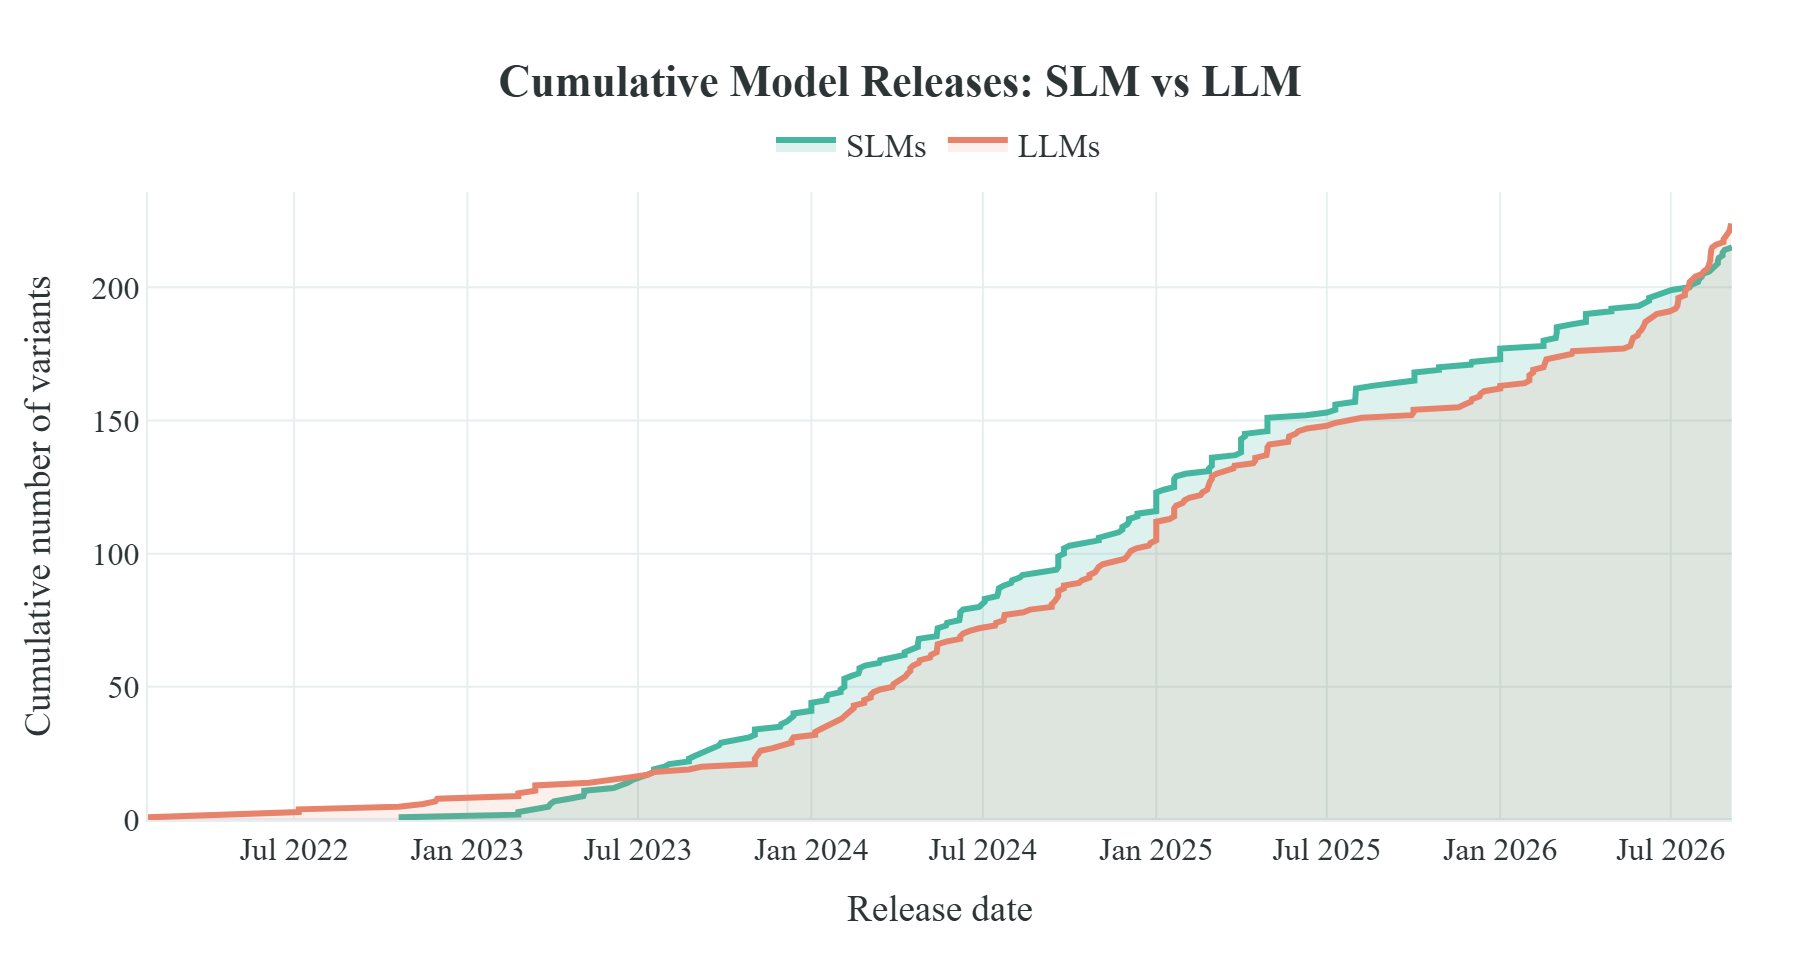
\includegraphics[width=\linewidth, alt={Two panels. Left: stacked bars of documented variants released per year from 2023 to 2026, split into small language models and small-active-parameter mixtures of experts; small language models peak at 71 in 2024 and fall to 51 in 2025 and 22 in 2026 to September, while small-active mixtures of experts rise to 19 in 2026. Right: cumulative release curves for small language models (reaching 179), small-active mixtures of experts (reaching 30), and large language models of disclosed size (reaching 104).}]{paper_combined_cumulative_releases.png}
  \caption{Documented variants by class: releases per year (left; 2026 to 4~September) and cumulative releases (right), from version~3.6 of the released inventory. SLMs meet both C1 and C2; small-active-parameter MoEs meet C1 only and are plotted separately; the comparison curve counts the 104 records of disclosed size that fail C1. The 119 records of undisclosed size cannot be classified and are not plotted.}
  \Description{Two panels. Left: stacked bars of documented variants released per year from 2023 to 2026, split into small language models and small-active-parameter mixtures of experts; small language models peak at 71 in 2024 and fall to 51 in 2025 and 22 in 2026 to September, while small-active mixtures of experts rise to 19 in 2026. Right: cumulative release curves for small language models (reaching 179), small-active mixtures of experts (reaching 30), and large language models of disclosed size (reaching 104).}
  \label{fig:cumulative_releases}
\end{figure}

% ----------------------------------------------------------------
\subsection{Definitions and Terminology}
\label{subsec:intro_definition}

``Small'' is used in the literature to mean at least four different things, so we fix the terms before using them.

\subsubsection{The Operative Definition}
\label{subsubsec:intro_def_operative}

A model is a \emph{small language model} in this survey when it satisfies both of the following:

\begin{description}
  \item[C1 (compute envelope)] It is an autoregressive decoder-only model (attention, state-space, or a hybrid) whose \emph{active} parameter count per generated token is at most roughly twenty billion.
  \item[C2 (storage envelope)] Its \emph{total} parameter count is also at most roughly twenty billion, so that its weights, about 11--15~GB at the 4.4--5.8 effective bits per weight of common 4-bit formats (\suppsec~\ref{subsec:reported_quantization}), can be stored and downloaded like a consumer application and, on runtimes that keep every weight in memory, held on one 16--24~GB consumer GPU or laptop.
\end{description}

\begin{figure}[t]
\centering
\footnotesize
\definecolor{dfInk}{HTML}{34404A}
\definecolor{dfBlue}{HTML}{7397B8}
\definecolor{dfLav}{HTML}{9B8FB5}
\definecolor{dfApr}{HTML}{D8A879}
\definecolor{dfSlate}{HTML}{A2AAB1}
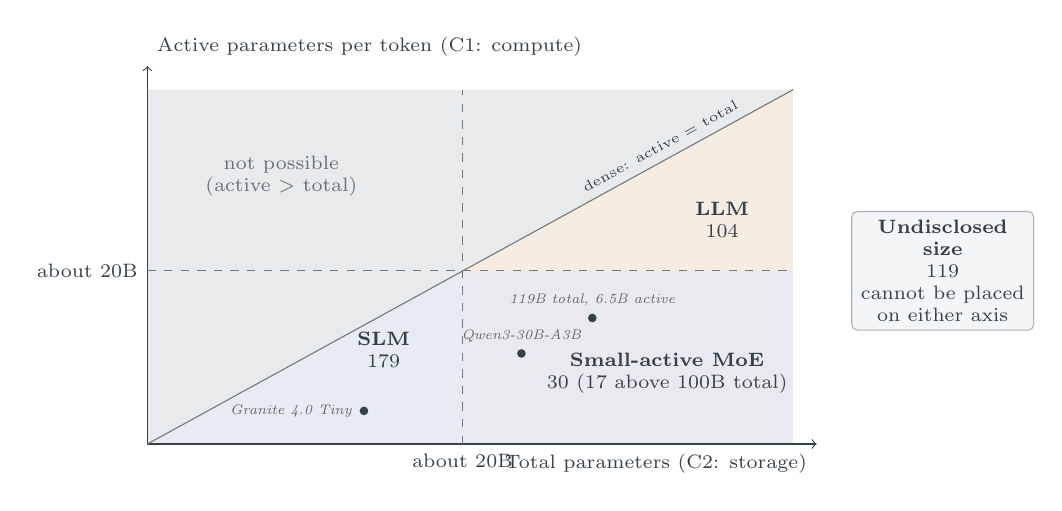
\begin{tikzpicture}[x=1cm,y=1cm,
  lab/.style={font=\scriptsize, text=dfInk, align=center},
  pt/.style={circle, fill=dfInk, inner sep=1.1pt},
  ptl/.style={font=\tiny\itshape, text=dfInk!80}]
% regions (axes: total parameters horizontally, active per token vertically; 20B at 4.0 / 2.2)
\fill[dfBlue!18] (0,0) -- (4.0,0) -- (4.0,2.2) -- cycle;
\fill[dfLav!20] (4.0,0) rectangle (8.2,2.2);
\fill[dfApr!22] (4.0,2.2) -- (8.2,2.2) -- (8.2,4.5) -- cycle;
\fill[dfSlate!25] (0,0) -- (8.2,4.5) -- (0,4.5) -- cycle;
% axes, threshold lines, diagonal
\draw[->, dfInk] (0,0) -- (8.5,0) node[below left, lab] {Total parameters (C2: storage)};
\draw[->, dfInk] (0,0) -- (0,4.8) node[above right, lab, anchor=south west] {Active parameters per token (C1: compute)};
\draw[dashed, dfInk!70] (4.0,0) -- (4.0,4.5);
\draw[dashed, dfInk!70] (0,2.2) -- (8.2,2.2);
\draw[dfInk!70] (0,0) -- (8.2,4.5);
\node[lab, below] at (4.0,0) {about 20B};
\node[lab, left] at (0,2.2) {about 20B};
\node[lab, rotate=28.8, above, font=\tiny] at (6.6,3.62) {dense: active $=$ total};
% region labels
\node[lab] at (3.0,1.2) {\textbf{SLM}\\179};
\node[lab] at (6.6,0.9) {\textbf{Small-active MoE}\\30 (17 above 100B total)};
\node[lab] at (7.3,2.85) {\textbf{LLM}\\104};
\node[lab, text=dfInk!75] at (1.7,3.4) {not possible\\(active $>$ total)};
% example models
\node[pt] at (2.75,0.42) {}; \node[ptl, left] at (2.72,0.42) {Granite 4.0 Tiny};
\node[pt] at (4.75,1.15) {}; \node[ptl, above] at (4.75,1.17) {Qwen3-30B-A3B};
\node[pt] at (5.65,1.6) {}; \node[ptl, above] at (5.65,1.62) {119B total, 6.5B active};
% undisclosed box
\node[draw=dfSlate!90, fill=dfSlate!12, rounded corners=2pt, lab, text width=21mm, inner sep=3pt] at (10.1,2.2) {\textbf{Undisclosed size}\\119\\cannot be placed on either axis};
\end{tikzpicture}
\caption{The two bounds of the definition. C1 bounds active parameters per token, which set per-token compute, latency, and energy; C2 bounds total parameters, which set storage and download size (and resident memory when every weight is kept in memory). Dense models lie on the diagonal. Counts are inventory records (version~3.6); example points are illustrative placements on schematic logarithmic axes, not a plot of the inventory.}
\Description{Schematic plane with total parameters on the horizontal axis and active parameters per token on the vertical axis, each with a threshold at about twenty billion. The region where both are below the threshold is labelled SLM, 179; below the active threshold but above the total threshold is small-active mixture of experts, 30, of which 17 exceed 100B total; above the active threshold is LLM, 104; above the diagonal is not possible. Example points: Granite 4.0 Tiny in the SLM region, Qwen3-30B-A3B and a 119B-total, 6.5B-active model in the small-active region. A separate box holds 119 records of undisclosed size.}
\label{fig:slm_definition}
\end{figure}

C1 bounds per-token compute, latency, and energy (Figure~\ref{fig:slm_definition}). C2 bounds storage and download size, and resident memory only on runtimes that keep all weights resident: runtimes that stream weights or experts from flash \citep{alizadeh2024llmflash}, as Apple's 20B-total, 1--4B-active on-device model does \citep{apple2026afm3}, decouple residency from total size, so for such models resident memory has to be reported separately rather than read off C2. The two conditions coincide for dense models, which is why a single threshold has sufficed in most prior work, but they come apart for \gls{moe} models: a 119B-total model that activates 6.5B parameters per token has the per-token cost of a 6.5B model and the storage cost of a 119B one. The twenty-billion figure is a convention, not a natural kind. Applied to the records of disclosed size in the released file, a bound of 10B, 13B, 20B, or 32B total parameters would admit 143, 160, 179, or 209 of them respectively, and every record carries its counts so that any other threshold can be applied.

\subsubsection{Four Distinguished Terms}
\label{subsubsec:intro_def_terms}

\begin{description}
  \item[\gls{slm}] A model satisfying C1 and C2. Every deployment, storage, and on-device claim in this paper applies to this class.
  \item[Compact model] An \gls{slm} at or below roughly 3B total parameters, whose 4-bit weights fit in about 2~GB of the 4--8~GB a current phone leaves to applications. Most documented phone deployments use this band; the exceptions keep part of the model off the accelerator, through per-layer embeddings (Gemma~3n and Gemma~4 E-series) or flash-resident experts (Apple's third-generation on-device model).
  \item[Edge model] A model, of any size, for which the developer documents and ships an artifact for phone-, single-board-computer-, or \gls{npu}-class hardware. ``Edge'' is a claim about the deployment target, not about parameter count.
  \item[Small-active-parameter \gls{moe}] A model satisfying C1 but not C2. These have \gls{slm}-like per-token cost and \gls{llm}-like storage cost. They are recorded in the inventory but counted, plotted, and discussed separately, and are excluded from every claim about storage, download size, resident memory, or on-device feasibility. The class is wide: 17 of its 30 members exceed 100B total parameters, so it includes frontier-scale models such as Llama~4 Maverick and Qwen3.5-397B-A17B as well as 21--35B models.
\end{description}

The inventory holds 179 \glspl{slm} and 30 small-active-parameter \glspl{moe}; wherever this paper counts \glspl{slm}, it means the 179. Per-layer-embedding ``effective'' sizes (Gemma~3n, Gemma~4 E2B/E4B) are not sparse activation, so C1 is evaluated on those models' total counts. The unit counted is the \emph{variant}: a separately released artifact of one size within a family, which may be a distinct post-training or domain specialization released as its own repository (for example Phi-4 and Phi-4-reasoning), with checkpoint revisions of the same artifact counted once. Counted instead by distinct family and size, the 179 \glspl{slm} are 136 family--size pairs. \suppsec~\ref{supp:definitions} lists the reporting dimensions the inventory records and their coverage (total parameters 209/209, context length 135/209, peak runtime memory not reported by vendors), and the artifact vocabulary.

\subsection{The Agentic Turn and the Thesis}
\label{subsec:intro_agentic}
\label{subsec:intro_thesis}

A large share of model calls is now issued by AI agents: control loops in which a model is called repeatedly to choose a tool, fill its arguments, extract a field, classify an intent, or check a result \citep{belcak2025slm_agentic,chen2024mas_survey}. Many such calls are narrow, repetitive, and format-constrained. \citet{belcak2025slm_agentic} argue that for these calls \glspl{slm} should be the default, and \citet{sharma2025slm_agentic} survey the evidence and propose an \gls{slm}-default, \gls{llm}-fallback design. We state the position as a conditional hypothesis whose terms can be measured.

\begin{quote}
\textbf{H (default hypothesis).} Consider a type of language-model call inside an agent with the following properties.
\begin{description}
  \item[H1 (bounded)] The output is a tool selection, a record conforming to a fixed schema, a label from a fixed set, or a local edit of a few lines.
  \item[H2 (recurrent)] The expected number of such calls over the planning horizon, $N$, exceeds the break-even volume
  \begin{equation}
    N^{*} = \frac{F}{\,c_L - (a\,c_S + c_V + e\,c_L)\,},
    \label{eq:breakeven}
  \end{equation}
  where $F$ is the one-time and maintenance cost of specializing for the call type, $c_L$ and $c_S$ are the per-call serving costs of the large and the small model, $a \ge 1$ is the expected number of small-model attempts per call, $c_V$ is the per-call cost of the check, and $e$ is the escalation rate. If the denominator is not positive, specialization never pays.
  \item[H3 (short-context)] The input needed fits within a few thousand tokens without retrieval over a large corpus.
  \item[H4 (checkable)] Two checks exist at a cost small relative to $c_L$: a \emph{validity} check (H4a: schema validation, parsing, type checking), and a \emph{correctness} check (H4b: an executor with observable effects, a unit test, a constraint solver, or a lookup against a reference) that detects outputs which are well formed but wrong. Validity checking alone does not satisfy H4.
\end{description}
For such a call type, a specialized \gls{slm} is the appropriate default: the call goes to the \gls{slm} first and is escalated to a frontier \gls{llm} when a check fails. ``Appropriate default'' means that the \gls{slm}-first system is non-inferior to an all-\gls{llm} system in task success, within a margin $\delta$ fixed in advance, at a lower cost per completed task than every comparator of Section~\ref{subsec:challenges_verification}.
\end{quote}

\begin{figure}[t]
\centering
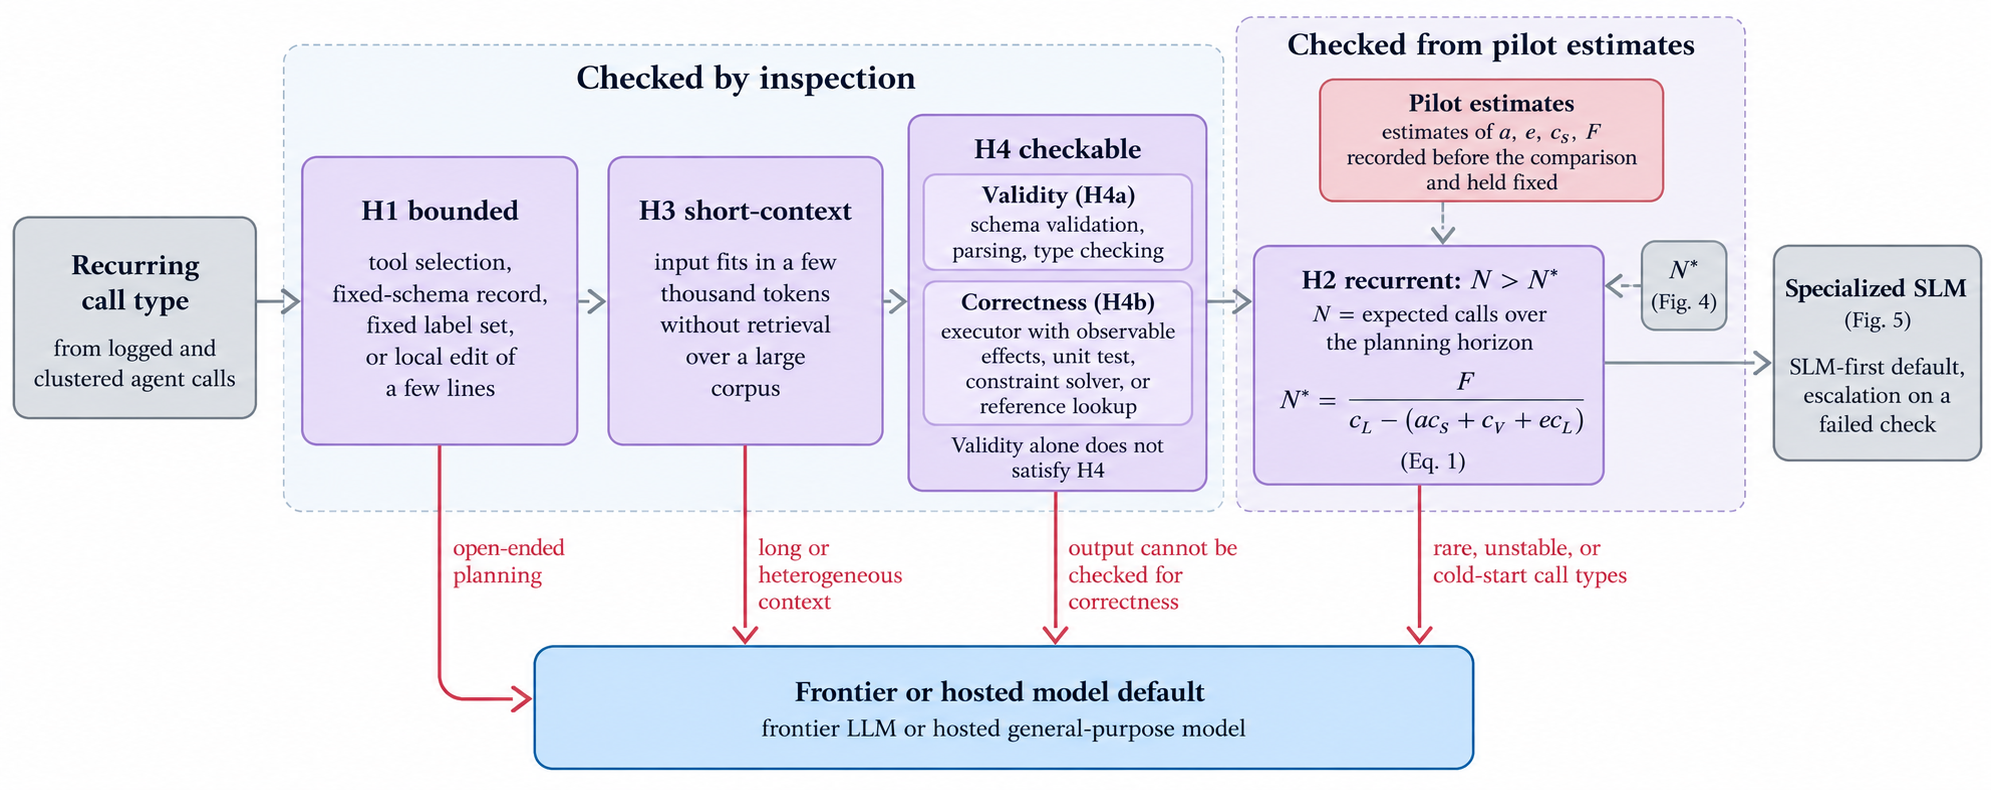
\includegraphics[width=\linewidth, alt={Left-to-right flow: a recurring call type passes through gates H1 bounded, H3 short-context, H4 checkable (validity and correctness), and H2 recurrent, and if all pass reaches specialized SLM as the default. From each gate a downward arrow labelled open-ended planning, long context, uncheckable output, or rare or unstable leads to a box reading frontier or hosted model as default. Labels mark H1, H3, and H4 as checked by inspection and H2 as checked from pilot estimates.}]{fig03-hypothesis-conditions.png}
\caption{Assessing one recurring agent call type against hypothesis~H at design time. H1, H3, and H4 are checked by inspecting the call type; H2 is checked against pilot estimates recorded before any comparison. A call type that passes every condition defaults to a specialized SLM with escalation on a failed check (Figure~\ref{fig:hetero_agent}); a failure at any condition, labelled with the workload class that typically fails there (Section~\ref{subsec:agentic_counterexamples}), leaves a frontier or hosted model as the default.}
\Description{Left-to-right flow: a recurring call type passes through gates H1 bounded, H3 short-context, H4 checkable (validity and correctness), and H2 recurrent, and if all pass reaches specialized SLM as the default. From each gate a downward arrow labelled open-ended planning, long context, uncheckable output, or rare or unstable leads to a box reading frontier or hosted model as default. Labels mark H1, H3, and H4 as checked by inspection and H2 as checked from pilot estimates.}
\label{fig:hypothesis_conditions}
\end{figure}

H1, H3, and H4 can be checked by inspecting a call type before any model is trained (Figure~\ref{fig:hypothesis_conditions}). H2 cannot be checked from first principles, because $a$, $e$, and $c_S$ depend on the specialized model: it is assessed from pilot estimates recorded before the comparison and held fixed, so that a failed comparison cannot be reclassified afterwards as a failure of H2. H is refuted for a workload class meeting H1--H4 if a pre-registered comparison of the kind specified in Section~\ref{subsec:challenges_verification} finds the \gls{slm}-first system inferior by more than $\delta$, or more costly per completed task than any comparator, and it is rejected as a general design rule if it fails on a majority of at least three pre-registered workloads with distinct call types. It does not claim that \glspl{slm} match frontier models in general, that agents can dispense with large models, or any particular share of agent traffic meeting H1--H4. Section~\ref{subsec:agentic_counterexamples} sets out the workload classes for which the conditions fail. Section~\ref{subsec:agentic_evidence} grades the evidence bearing on H: it is strongest for per-call competence of specialized sub-10B models, contested for end-to-end success, and absent for cost per completed task in an \gls{slm}-first agent.

\subsection{Scope and Contributions}
\label{subsec:intro_gap}

Existing \gls{slm} surveys \citep{lu2024slmsurvey,vannguyen2024slm_survey,wang2024comprehensive,gupta2025slmsurvey} provide taxonomies, technique reviews, and measurements but treat agentic deployment only in passing. The agentic case has been made as a position \citep{belcak2025slm_agentic,tian2026edgeagents} and as a survey \citep{sharma2025slm_agentic}, which already proposes \gls{slm}-default, \gls{llm}-fallback systems with verifier cascades, cost per successful task as the deciding metric, and limits where fallback remains necessary. We share that direction. This paper adds the following:

\begin{description}
  \item[A two-bound definition] that separates per-token cost (C1) from storage cost (C2) and so treats mixtures of experts consistently (Section~\ref{subsec:intro_definition}).
  \item[A verified inventory] of 179 \glspl{slm} and 30 small-active-parameter \glspl{moe} (2023--2026), in which every record's developer source has been checked and every inclusion decision is recorded with its reason, released with the scripts that apply the rule and generate every table and figure (\suppsec~\ref{supp:method}).
  \item[An audit of the vendor evaluation record] that quantifies why a cross-model table cannot be built from it: for the 14 cohort models of the four largest vendors, no benchmark is reported for all of them, and no stated protocol is shared by more than five (Section~\ref{sec:reported}).
  \item[A compression review] that reports reductions along separate axes of parameters, memory, training compute, and latency (Section~\ref{sec:compression}).
  \item[An operational version of the agentic hypothesis] with a break-even condition that includes retries, checking, and escalation, a correctness requirement on the check, graded agent-specific evidence including contrary results, and the workload classes for which it fails (Section~\ref{sec:agentic}).
  \item[A falsification design] that specifies comparators, the statistical decision rule, and the sample size needed to decide H for a workload, with five further verification studies (Section~\ref{sec:challenges}).
\end{description}

\subsection{Survey Method and Sources}
\label{subsec:intro_method}

This is a structured narrative survey, not a systematic review; its aims are representative coverage of the design space, a verified inventory, and an audit of a defined cohort. It addresses five research questions: the design space of \glspl{slm} released 2023--2026 (RQ1); which compression techniques pay in the sub-10B regime, along which axis, and at what quality cost (RQ2); what the vendor evaluation record can and cannot support (RQ3); what agent-specific evidence says about small models (RQ4); and under which conditions a small model is the appropriate default inside an agent (RQ5).
\label{subsubsec:intro_rqs}
\label{subsubsec:intro_search}

\emph{Model inventory (RQ1).} A seed list compiled in March 2026 from public model listings and aggregators, 205 of whose records were compiled with the assistance of a large language model, was updated on 5~September 2026 against the OpenRouter catalogue and vendor announcements, and every record was then classified against C1 and C2. On 8~October 2026 every record's developer source was checked through the Hugging Face Hub API: 197 of the 209 included records link an existing repository owned by the developer, and the other 12 link the developer's own announcement, paper, or code repository. Twelve records first sourced from an aggregator or a press article were re-sourced to the developer, and one for which no developer source exists was excluded. C1, C2, and inclusion criteria M1 (a developer source states size and architecture) and M4 (a dated release) are computed from recorded fields by a released script; the exclusions of derivative fine-tunes, API aliases, and encoder-decoder models are named editorial decisions listed in that script. The released file records, per record, the check, its date, and the Hub parameter count where available. Coverage is strongest for developers that publish on the Hub. \suppsec~\ref{supp:method} gives the criteria, the seven excluded records, and the count history.

\emph{Technique literature (RQ2, RQ4, RQ5).} Works were identified from the prior surveys cited above, by backward and forward citation tracing, and by targeted searches of arXiv and the ACL Anthology, last run on 8~October 2026 for agent-specific evaluation, routing, function calling, and cost-per-outcome measurement. Screening decisions were not recorded for this stream, so statements that we ``found no'' study are bounded by that search.

\emph{Evaluation record (RQ3).} For each model of the 18-model cohort, the primary release document and official model card were consulted; the coverage ledger of Section~\ref{subsec:reported_overall} was transcribed from them on 8~October 2026. No benchmark was executed for this survey.

\emph{Appraisal.} Each empirical claim carries an evidence grade (Section~\ref{subsec:reported_grading}) reflecting its design and the independence of its source.
\label{subsubsec:intro_inclusion_summary}

\subsection{Organization}
\label{subsec:intro_organization}

Section~\ref{section:background} reviews related work. Section~\ref{sec:taxonomy} presents the taxonomy, Section~\ref{sec:compression} compression, Section~\ref{sec:reported} the evaluation record and the grading scheme, and Section~\ref{sec:deployment} deployment. Section~\ref{sec:agentic} assesses H on agent-specific evidence and states its counterexamples. Section~\ref{section:discussion} discusses implications, applications, and limitations, Section~\ref{sec:challenges} sets out open problems and the verification agenda, and Section~\ref{section:conclusion} concludes. The electronic supplement (\suppsec~\ref{supp:definitions} to \suppsec~\ref{supp:last}) holds the reporting dimensions, inclusion criteria and released artifacts, detailed technique reviews, the audit ledger, reference tables, domain applications, and the generated variant inventory.
